%% chapter7_slides.tex  -  Chapter 7: Bayesian Detection of Recovery on Charged-Off Loan Accounts
%% Bayesian Machine Learning in Quantitative Finance: Theory and Practical Applications
%% Mongwe, Mbuvha & Marwala (Springer, 2025)
%% Compile: pdflatex -interaction=nonstopmode chapter7_slides.tex  (twice)
\documentclass[aspectratio=169,10pt]{beamer}

\usetheme{Madrid}
\usecolortheme{seahorse}
\usefonttheme{professionalfonts}

%% packages
\usepackage{amsmath,amssymb,mathtools}
\usepackage{bm}
\usepackage{graphicx}
\usepackage{booktabs}
\usepackage{array}
\usepackage{listings}
\usepackage{xcolor}

\graphicspath{{figures/}}

%% listings style
\lstdefinestyle{pycode}{
  language=Python,
  basicstyle=\ttfamily\scriptsize,
  keywordstyle=\color{blue!70!black}\bfseries,
  commentstyle=\color{green!50!black}\itshape,
  stringstyle=\color{orange!80!black},
  numbers=left,
  numberstyle=\tiny\color{gray},
  numbersep=5pt,
  frame=single,
  backgroundcolor=\color{gray!7},
  tabsize=2,
  showstringspaces=false,
  breaklines=true,
  captionpos=b,
}
\lstset{style=pycode}

%% footline, no navigation symbols
\setbeamertemplate{footline}[frame number]
\setbeamertemplate{navigation symbols}{}

%% macros
\newcommand{\R}{\mathbb{R}}
\newcommand{\Exp}{\mathbb{E}}
\newcommand{\Prob}{\mathbb{P}}
\newcommand{\bw}{\mathbf{w}}
\newcommand{\bp}{\mathbf{p}}
\newcommand{\bx}{\mathbf{x}}

%%=============================================================================
\title[Bayesian ML in QF -- Ch.7]{Bayesian Machine Learning in Quantitative Finance}
\subtitle{Chapter 7: Recovery on Charged-Off Loan Accounts}
\author{Based on Mongwe, Mbuvha \& Marwala}
\date{}

%%=============================================================================
\begin{document}

\begin{frame}
  \titlepage
\end{frame}

\begin{frame}{Chapter Outline}
  \tableofcontents
\end{frame}

%%=============================================================================
\section{7.1 Introduction}
%%=============================================================================

\begin{frame}[allowframebreaks]{The Business Problem: Charge-Offs and Recoveries}

\textbf{Plain-language setup.} A bank lends money. If a borrower stops repaying and the loan is deemed uncollectable through normal servicing, the lender \emph{charges off} (writes off) the loan as a loss on its books. But charging off is an accounting decision, not the end of the story: the lender (or whoever now owns the debt) may still pursue the borrower --- letters, calls, payment-plan negotiations, or legal action --- and \textbf{recover some fraction of the money later}.

\begin{alertblock}{The Business Problem in One Sentence}
Given everything known about a defaulted account at charge-off, \emph{will there be a meaningful recovery, and how much}? Getting this right lets a bank (or whoever buys the distressed debt) price the loan book correctly and target collections effort efficiently.
\end{alertblock}

\begin{block}{Key Credit-Risk Quantities}
\begin{itemize}
  \item \textbf{Recovery rate} = (amount eventually collected $-$ administrative cost of collecting it) $/$ (exposure at default, i.e.\ the outstanding balance when the loan defaulted).
  \item \textbf{Loss given default (LGD)} $= 1 - $ recovery rate: the fraction of the exposure the lender never gets back.
  \item \textbf{Probability of default (PD)} and \textbf{exposure at default (EAD)} are the other two pillars of credit-risk modelling; together PD, LGD, EAD drive a bank's regulatory capital requirements (Basel III's internal-ratings-based approach lets a bank estimate LGD itself, which is why getting LGD/recovery modelling right matters commercially, not just academically).
\end{itemize}
\end{block}

\framebreak

\begin{block}{Why This Is a Hard Modelling Problem}
Empirically, the distribution of recovery rates is strongly bimodal/skewed: a large mass of accounts recover (close to) nothing, and a smaller mass recovers (close to) everything, with everything else spread thinly in between. A single smooth regression model tends to fit this poorly -- ``one size fits all'' does not work well here.
\end{block}

\begin{block}{Prior Work (Non-Bayesian and Bayesian)}
\begin{itemize}
  \item Bellotti \& Crook (2012): Tobit and decision-tree models, Beta/fractional-logit transforms of the recovery rate on UK credit-card defaults -- plain OLS with macroeconomic variables actually forecast best.
  \item Calabrese (2014): a mixed continuous-discrete model with a Beta random variable for the continuous part of the recovery rate (Bank of Italy data).
  \item Loterman et al. (2012): a 24-model benchmark across six bank datasets -- non-linear models (e.g.\ neural networks) beat linear ones.
  \item Ye \& Bellotti (2019): a two-stage Beta-mixture + logistic-regression model that captures the multi-modal recovery-rate shape.
  \item Zhang \& Zhao (2024): the first to use \emph{MCMC sampling} to draw model coefficients and generate LGD distributions -- a Bayesian approach, but not one that studies MCMC \emph{algorithm choice} itself.
\end{itemize}
\end{block}

\framebreak

\begin{block}{This Chapter's Contribution}
\begin{itemize}
  \item First use of \textbf{Bayesian logistic regression with an automatic relevance determination prior (BLR-ARD)} to detect the \emph{presence} of recovery on charged-off loans, using real peer-to-peer lending data.
  \item Being Bayesian means every prediction carries an uncertainty quantification, and the ARD prior automatically ranks which input features matter (with uncertainty on that ranking too) -- more interpretable for stakeholders than a black-box point estimate.
  \item MCMC is used to train the model because it is \emph{asymptotically exact}: unlike variational inference or the Laplace approximation, a properly run MCMC chain converges to the \emph{true} posterior, not an approximation to it.
  \item Three MCMC samplers are compared for training BLR-ARD, introduced in this chapter for the first time in this modelling context: \textbf{MALA}, \textbf{HMC}, and the \textbf{No-U-Turn Sampler (NUTS)}.
\end{itemize}
\end{block}

\end{frame}

%%=============================================================================
\section{7.2 Model for Bayesian Detection of Recoveries}
%%=============================================================================

\begin{frame}[allowframebreaks]{7.2 Bayesian Logistic Regression for Recovery Detection}

\textbf{Intuition.} We want to predict a \emph{binary} outcome -- did this charged-off account recover a meaningful amount, yes or no? Logistic regression is the natural workhorse for binary outcomes; the Bayesian wrapper around it gives us a full posterior over the coefficients (hence uncertainty) instead of one point estimate, and the ARD prior additionally tells us which features actually drive that prediction.

\begin{block}{Negative Log-Likelihood of the Logistic Model (Eq.~7.1)}
\[
  l(\mathrm{D}\mid \bw) = \sum_{i}^{N} y_i \log(\bw^T x_i) + (1-y_i)\log(1-\bw^T x_i)
\]
\textbf{Symbols:} $\mathrm{D} = \{\bx, y\}$ is the data (features and binary labels); $N$ is the number of observations; $\bw$ is the vector of coefficients to be estimated; $y_i \in \{0,1\}$ is the observed outcome for account $i$ (here: ``recovered more than 10\%?''); $x_i$ is the feature vector for account $i$. As usual for logistic regression, $\bw^T x_i$ is understood to be passed through the logistic sigmoid $\sigma(z) = 1/(1+e^{-z})$ to produce a valid probability before taking the logarithm.
\end{block}

\begin{block}{Un-normalised Log-Posterior (Eq.~7.2)}
\[
  \ln p(\bw \mid \mathrm{D}) = l(\mathrm{D}\mid \bw) + \ln p(\bw \mid \alpha) + \ln q(\alpha)
\]
\textbf{Symbols:} $\ln p(\bw\mid\alpha)$ is the log-prior on the coefficients given hyperparameters $\alpha$; $\ln q(\alpha)$ is the log-distribution of the hyperparameters themselves. This is the quantity MALA/HMC/NUTS will draw samples from (up to a constant), i.e.\ the target of MCMC.
\end{block}

\framebreak

\begin{block}{The Automatic Relevance Determination (ARD) Prior}
Each coefficient $w_i$ gets a zero-mean Gaussian prior with \emph{its own} variance $\alpha_i$:
\[
  w_i \sim \mathcal{N}(0, \alpha_i)
\]
\textbf{Intuition:} $\alpha_i$ is a learned ``volume knob'' per feature. A large $\alpha_i$ lets $w_i$ range far from zero, i.e.\ the model is allowed to make feature $i$ influential; a small $\alpha_i$ squeezes $w_i$ toward zero, i.e.\ the model effectively switches feature $i$ off. Because we infer $\alpha_i$ for every feature jointly with $\bw$, the model \emph{automatically ranks feature importance} as a by-product of Bayesian inference -- no separate feature-selection step is needed.
\end{block}

\begin{block}{Jointly Sampling $\bw$ and $\alpha$}
The $\alpha_i$ are assumed log-normally distributed with mean zero and unit variance. Rather than alternating between sampling $\bw$ and $\alpha$ in a Gibbs scheme, this chapter samples $\bw$ and $\alpha$ \emph{jointly} in one MCMC step. This doubles the dimensionality of the space being explored, but empirically gives more stable exploration across all three MCMC methods compared here.
\end{block}

\end{frame}

\begin{frame}[fragile]{Python: Toy Loan Dataset \& BLR-ARD Log-Posterior}
\begin{lstlisting}[caption={A tiny illustrative "loan recovery" dataset and the BLR log-posterior building blocks (author's toy code, not the book's)}]
import numpy as np

# 6 FICTIONAL charged-off accounts: days-since-default, outstanding
# balance, and "recovered more than 10%?" (mirrors the book's binary
# target definition in Sect. 7.4.2) -- all numbers made up for illustration
days_since_default  = np.array([30, 400, 90, 250, 600, 150.0])
outstanding_balance = np.array([500, 8000, 1200, 4000, 12000, 2500.0])
recovered_gt_10pct  = np.array([1, 0, 1, 0, 0, 1.0])

# standardise features, add intercept column
x1 = (days_since_default  - days_since_default.mean())  / days_since_default.std()
x2 = (outstanding_balance - outstanding_balance.mean()) / outstanding_balance.std()
X = np.column_stack([np.ones_like(x1), x1, x2])
y = recovered_gt_10pct

def sigmoid(z):
    return 1.0 / (1.0 + np.exp(-z))

def log_posterior(w, X, y, prior_var):
    """Eq. 7.1 (logistic log-lik) + Eq. 7.2 (Gaussian/ARD-style log-prior)."""
    p = np.clip(sigmoid(X @ w), 1e-9, 1 - 1e-9)
    loglik  = np.sum(y * np.log(p) + (1 - y) * np.log(1 - p))
    logprior = -0.5 * np.sum(w**2) / prior_var   # w_i ~ N(0, alpha_i), alpha_i=prior_var here
    return loglik + logprior
\end{lstlisting}
\end{frame}

%%=============================================================================
\section{7.3 Markov Chain Monte Carlo Algorithms}
%%=============================================================================

\begin{frame}{Notation You'll Need / Recap}
You have already seen MALA and HMC derived in detail (Chapter 3 of this book series). Here we give an \emph{efficient} recap of both, then spend most of our time on what is \textbf{new}: the No-U-Turn Sampler (NUTS).

\begin{block}{The One-Line Idea Behind Each Method}
\begin{itemize}
  \item \textbf{MALA}: random-walk Metropolis-Hastings, but nudged by the gradient of the log-posterior (steepest-ascent drift + noise), corrected by an accept/reject step.
  \item \textbf{HMC}: introduce a fictitious ``momentum'' variable and simulate deterministic (Hamiltonian) physics for several steps to make a distant, low-autocorrelation proposal, corrected by an accept/reject step.
  \item \textbf{NUTS}: HMC, but with \emph{no user-chosen trajectory length} -- the algorithm figures out for itself, on every iteration, how far to simulate before stopping.
\end{itemize}
\end{block}
\end{frame}

%%-----------------------------------------------------------------------------
\subsection{7.3.1 Metropolis-Adjusted Langevin Algorithm}
%%-----------------------------------------------------------------------------

\begin{frame}[allowframebreaks]{7.3.1 MALA -- Efficient Recap}

\textbf{Intuition (quick recap).} Plain random-walk Metropolis-Hastings proposes blindly in every direction. MALA instead nudges the proposal \emph{uphill} along the gradient of the log-target before adding noise, so proposed points are more likely to land somewhere probable -- fewer wasted, rejected moves.

\begin{block}{Langevin Diffusion (Eq.~7.3)}
\[
  d\bw_t = \tfrac{1}{2} f'(\bw)\, dt + dZ_t
\]
\textbf{Symbols:} $\bw$ are the parameters being sampled; $f'(\bw)$ is the first derivative (gradient) of the target log-density $f(\bw)$ w.r.t.\ $\bw$; $Z_t$ is a Brownian-motion process in fictitious time $t$. This continuous-time process, if we could simulate it exactly, would have the target as its stationary distribution.
\end{block}

\begin{block}{Why the Metropolis Correction Is Needed}
The diffusion in Eq.~7.3 usually cannot be solved analytically, so we discretise it (e.g.\ Euler-Maruyama). Discretisation introduces error that can break detailed balance, so an MH accept/reject step is bolted on afterward to guarantee convergence to the correct target. MALA converges faster than plain MH (thanks to the gradient information) but its samples remain noticeably autocorrelated -- this motivates HMC, which takes multiple correlated micro-steps per proposal instead of just one.
\end{block}

\end{frame}

\begin{frame}[fragile]{Python: From-Scratch MALA Sampler (Toy Running Example)}
\begin{lstlisting}[caption={A minimal MALA sampler for the toy BLR posterior of the loan-recovery example}]
def grad_log_posterior(w, X, y, prior_var):
    p = sigmoid(X @ w)
    grad_loglik  = X.T @ (y - p)      # d/dw of Eq. 7.1
    grad_logprior = -w / prior_var    # d/dw of Gaussian ARD-style prior
    return grad_loglik + grad_logprior

def run_mala(X, y, n_iter=12000, burn_in=2000, step=1.6, prior_var=5.0, seed=0):
    rng = np.random.default_rng(seed)
    w = np.zeros(X.shape[1])
    samples, n_accept = np.zeros((n_iter, X.shape[1])), 0
    for t in range(n_iter):
        grad = grad_log_posterior(w, X, y, prior_var)
        # Langevin proposal: drift + Gaussian noise (discretised Eq. 7.3)
        w_prop = w + 0.5*step**2*grad + step*rng.normal(size=X.shape[1])
        grad_prop = grad_log_posterior(w_prop, X, y, prior_var)
        # MH correction accounts for the asymmetric proposal density
        fwd = w_prop - w - 0.5*step**2*grad
        bwd = w - w_prop - 0.5*step**2*grad_prop
        log_alpha = (log_posterior(w_prop, X, y, prior_var) - 0.5*np.sum(fwd**2)/step**2
                   - log_posterior(w,      X, y, prior_var) + 0.5*np.sum(bwd**2)/step**2)
        if np.log(rng.uniform()) < log_alpha:
            w = w_prop; n_accept += 1
        samples[t] = w
    return samples[burn_in:], n_accept / n_iter   # kept samples, acceptance rate
\end{lstlisting}
\end{frame}

\begin{frame}{Toy Running Example: MALA Diagnostics}

\textbf{Reminder:} this is the author's own illustrative simulation on 6 fictional charged-off accounts -- not the book's Lending Club results (those come in Sect.~7.5).

\begin{center}
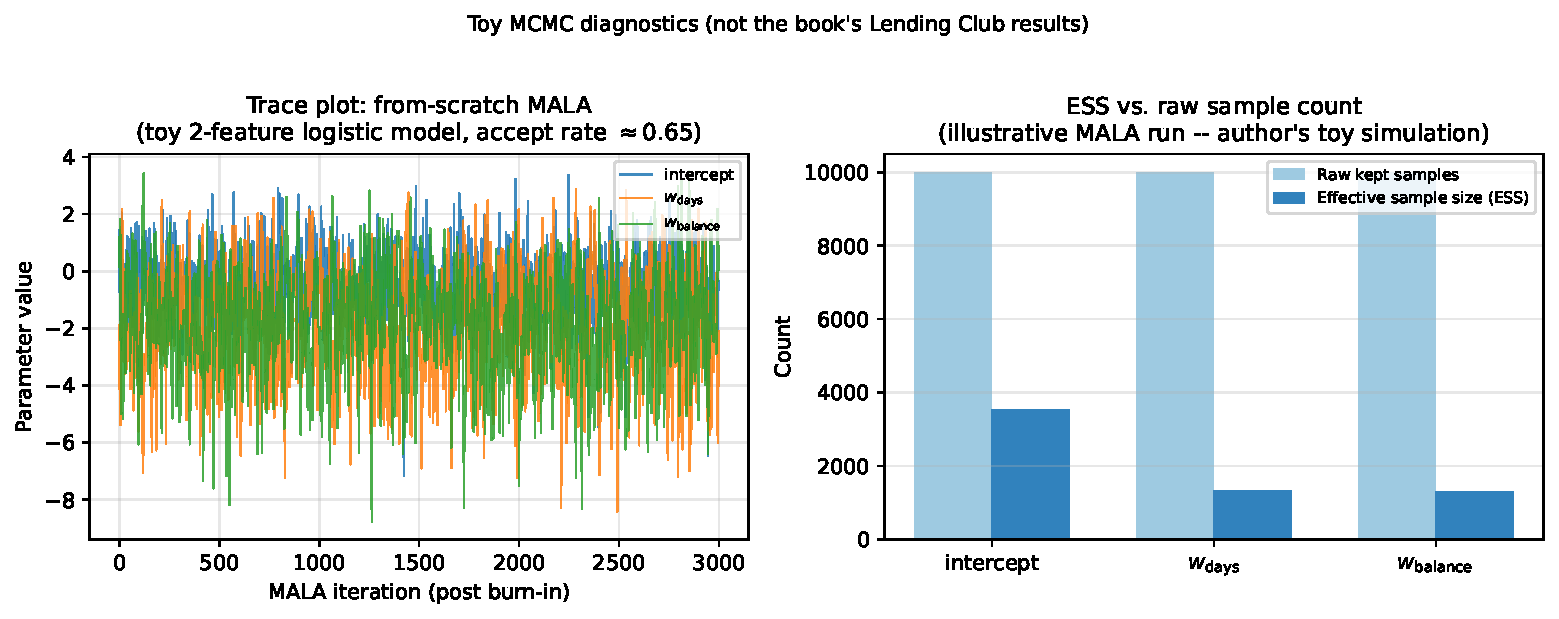
\includegraphics[width=0.95\linewidth]{fig_mcmc_diagnostics.pdf}
\end{center}

With a step size tuned toward the book's $\sim$60\% MALA target acceptance rate, the trace plots mix but still show visible autocorrelation, and the effective sample size (ESS) is well below the raw number of kept iterations -- exactly the "samples are still correlated" behaviour the book describes for MALA on the real dataset.
\end{frame}

%%-----------------------------------------------------------------------------
\subsection{7.3.2 Hamiltonian Monte Carlo and the No-U-Turn Sampler}
%%-----------------------------------------------------------------------------

\begin{frame}[allowframebreaks]{7.3.2 HMC -- Efficient Recap}

\textbf{Intuition (quick recap).} Treat $-\log(\text{posterior})$ as a landscape of potential energy. Give the parameter a fictitious momentum $\bp$ and let it slide around this landscape following the laws of physics (Hamiltonian dynamics) for a while before stopping -- because physics conserves energy, the proposal can travel \emph{far} from its start while staying in high-probability territory, dramatically cutting autocorrelation relative to MALA/MH.

\begin{block}{Hamiltonian Dynamics (Eq.~7.4)}
\[
  \frac{d\bw}{dt} = \frac{\partial H(\bw,\bp)}{\partial \bp}, \qquad
  \frac{d\bp}{dt} = -\frac{\partial H(\bw,\bp)}{\partial \bw}
\]
\textbf{Symbols:} $\bw$ are the parameters; $\bp$ is an auxiliary momentum variable of the same dimension as $\bw$; $H(\bw,\bp)$ is the Hamiltonian (total energy) = potential energy (from the target posterior) + kinetic energy (typically a multivariate Gaussian in $\bp$).
\end{block}

\begin{block}{Leapfrog Integration (Eq.~7.5) and MH Correction (Eq.~7.6)}
\[
  \bp_{t+\epsilon/2} = \bp_t + \tfrac{\epsilon}{2}\tfrac{\partial H}{\partial \bw},\quad
  \bw_{t+\epsilon} = \bw_t + \epsilon \mathbf{M}^{-1}\bp_{t+\epsilon/2},\quad
  \bp_{t+\epsilon} = \bp_{t+\epsilon/2} + \tfrac{\epsilon}{2}\tfrac{\partial H}{\partial \bw}
\]
\[
  \Prob(\text{accept } \bw^*) = \min\!\left(1, \frac{\exp(-H(\bw^*,\bp^*))}{\exp(-H(\bw,\bp))}\right)
\]
\textbf{Symbols:} $\epsilon$ is the discretisation (leapfrog) step size; $\mathbf{M}$ is a covariance ("mass") matrix in the kinetic-energy term. Two nested steps: (1) leapfrog-integrate the dynamics for some number of steps -- this is the \emph{trajectory length}; (2) MH-correct for the leapfrog's numerical error. When trajectory length $=1$, HMC collapses exactly to MALA.
\end{block}

\framebreak

\begin{block}{The Tuning Headache HMC Leaves Behind}
HMC has two knobs: step size $\epsilon$ and trajectory length (number of leapfrog steps $L$).
\begin{itemize}
  \item Step size: too small $\to$ correlated samples, wasted computation; too large $\to$ large discretisation error, low acceptance. Usually tuned via dual averaging toward a target acceptance rate.
  \item Trajectory length: too short $\to$ HMC degenerates into random-walk-like behaviour (losing its whole advantage); too long $\to$ the simulated path \emph{U-turns} and retraces itself, wasting expensive gradient evaluations without adding new information.
\end{itemize}
Tuning both well typically needs multiple costly pilot runs. \textbf{This is exactly the gap NUTS closes.}
\end{block}

\end{frame}

\begin{frame}{NUTS in Plain Terms}

\begin{alertblock}{The Core Idea}
HMC needs you to choose how many leapfrog steps to simulate -- too few wastes the method's power (it barely escapes a random walk), too many wastes computation retracing your steps (the trajectory curves back on itself). \textbf{NUTS automatically figures out when to stop} by detecting the moment the simulated path starts ``curving back'' on itself -- a U-turn -- so the user never has to hand-pick a trajectory length.
\end{alertblock}

\begin{block}{What NUTS Tunes Automatically}
\begin{itemize}
  \item \textbf{Step size $\epsilon$}: adapted during an initial burn-in/warm-up phase via primal-dual averaging, targeting a user-specified MH acceptance rate $\delta$.
  \item \textbf{Trajectory length}: adapted \emph{every iteration} by growing the simulated path until it either detects a U-turn or the Hamiltonian numerically diverges.
\end{itemize}
Result: NUTS performs at least as efficiently as a well-tuned standard HMC, and often better, \emph{without} the costly pilot-tuning runs HMC needs -- making it accessible to non-expert users.
\end{block}

\end{frame}

\begin{frame}[allowframebreaks]{Step-Size Adaptation: Primal-Dual Averaging}

\textbf{Intuition.} We want the chain's actual acceptance rate to hover near a target $\delta$ (e.g.\ 0.8) automatically, without manual trial and error, during the burn-in/warm-up window.

\begin{block}{Dual-Averaging Update (Eq.~7.7)}
\[
  \epsilon_{t+1} \leftarrow \mu - \frac{\sqrt{t}}{\gamma}\frac{1}{t+t_0}\sum_{i=1}^{t} H_i,
  \qquad
  \bar\epsilon_{t+1} \leftarrow \eta_t \epsilon_{t+1} + (1-\eta_t)\bar\epsilon_t
\]
\textbf{Symbols:} $\eta_t$ is a decaying adaptation-rate schedule; $\gamma$ regulates how strongly $\epsilon_t$ is pulled toward $\mu$; $H_t$ is the running difference between the target and actual acceptance rate up to step $t$; $\mu$ is a free parameter (an anchor value) that $\epsilon_t$ gravitates toward; $\bar\epsilon_t$ is an averaged, smoothed version of the step size used once warm-up ends.
\end{block}

\begin{block}{The Zero-in-Expectation Condition (Eq.~7.8)}
\[
  \Exp[H_t] = \Exp[\delta - \alpha_t] = 0
\]
\textbf{Symbols:} $\delta$ is the target MH acceptance rate; $\alpha_t$ is the actual acceptance probability at step $t$. This says the step size should be adapted so that, on average, the realised acceptance rate matches the target exactly.
\end{block}

\framebreak

\begin{block}{Recommended Settings (used in this chapter, from Hoffman \& Gelman, 2014)}
\[
  \mu = \log(10\epsilon_0), \quad \bar\epsilon_0 = 1, \quad \bar H_0 = 0, \quad \gamma = 0.05, \quad t_0 = 10, \quad \kappa = 0.75, \quad \epsilon_0 = 0.0001
\]
These give acceptable performance across a wide variety of target posteriors, and are exactly the settings used later in this chapter's numerical experiments for both HMC and NUTS.
\end{block}

\end{frame}

\begin{frame}{The NUTS Stopping Criterion: The U-Turn / Doubling Procedure}

\textbf{Intuition first.} Rather than pre-committing to a trajectory length, NUTS grows a trajectory outward from the current point in a tree-doubling fashion, and stops the instant the path shows signs of turning back toward where it started.

\begin{block}{Step-by-Step Outline}
\begin{enumerate}
  \item \textbf{Initialise:} start with a single point (current $\bw$, freshly sampled momentum $\bp$) -- a trivial trajectory of length $2^0=1$.
  \item \textbf{Double:} at each round, flip a coin to extend the trajectory either forward or backward in fictitious time, taking that many leapfrog steps to double the trajectory built so far ($1, 2, 4, 8,\dots$ steps).
  \item \textbf{Check for a U-turn:} after each doubling, test whether the vector between the leftmost and rightmost points of the (sub-)trajectory, dotted with the momentum at either end, has become non-positive: $(\bw^{+} - \bw^{-})\cdot \bp^{-} \le 0$ or $(\bw^{+}-\bw^{-})\cdot \bp^{+} \le 0$. A non-positive value means the path has stopped moving away from its start -- it is curving back.
  \item \textbf{Check for divergence:} also stop doubling if the simulated Hamiltonian has blown up numerically, which signals the step size was too large for this trajectory.
  \item \textbf{Stop / continue:} stop doubling as soon as step 3 or step 4 triggers anywhere in the (sub-)tree; otherwise keep doubling.
  \item \textbf{Select the next sample:} from the whole valid trajectory just built, draw the next sample using a slice-sampling technique over the visited states -- this extra device is needed because the adaptive, random stopping time would otherwise break detailed balance.
\end{enumerate}
\end{block}

\end{frame}

\begin{frame}[fragile]{Python: Illustrative Leapfrog Step + U-Turn Check}
\begin{lstlisting}[caption={Toy leapfrog integrator and a NUTS-style U-turn test (illustrative, simplified -- omits the full recursive doubling tree and slice sampling for brevity)}]
def leapfrog(w, p, grad_fn, eps):
    """One leapfrog step implementing Eq. 7.5."""
    p_half = p + 0.5 * eps * grad_fn(w)
    w_new  = w + eps * p_half            # here M = identity for simplicity
    p_new  = p_half + 0.5 * eps * grad_fn(w_new)
    return w_new, p_new

def is_u_turn(w_minus, w_plus, p_minus, p_plus):
    """Implements the U-turn test used inside NUTS' doubling procedure."""
    delta = w_plus - w_minus
    return (delta @ p_minus <= 0) or (delta @ p_plus <= 0)

def grow_trajectory_toy(w0, p0, grad_fn, eps, max_doublings=10):
    """Illustrative (non-recursive) doubling loop: grow until U-turn."""
    w_minus, w_plus, p_minus, p_plus = w0, w0, p0, p0
    trajectory = [w0]
    for j in range(max_doublings):
        direction = np.random.choice([-1, 1])
        n_new_steps = 2 ** j
        for _ in range(n_new_steps):
            if direction == 1:
                w_plus, p_plus = leapfrog(w_plus, p_plus, grad_fn, eps)
                trajectory.append(w_plus)
            else:
                w_minus, p_minus = leapfrog(w_minus, p_minus, grad_fn, -eps)
                trajectory.append(w_minus)
        if is_u_turn(w_minus, w_plus, p_minus, p_plus):
            break                              # stop: path is curving back
    return trajectory   # a real NUTS would slice-sample the next w from this
\end{lstlisting}
\end{frame}

%%=============================================================================
\section{7.4 Numerical Experiments}
%%=============================================================================

\begin{frame}[allowframebreaks]{7.4.1 Data Description}

\textbf{Setting:} recovery-rate data on charged-off loans from the \emph{Lending Club} peer-to-peer lending platform, 2018 vintage.

\begin{block}{Dataset at a Glance}
\begin{itemize}
  \item 658 records total; 70-30 train-test split.
  \item 43 candidate input variables spanning: balances and utilisation (e.g.\ total current balance, revolving balance, balance-to-limit ratio), credit-bureau inquiry counts, account counts and delinquency history, loan terms (amount, interest rate, term, instalment, purpose, grade/sub-grade), and borrower demographics (state, employment length, home ownership, annual income).
  \item The recovery-rate distribution is heavily right-skewed: the large majority of charged-off accounts recover close to nothing, with a secondary small cluster around 10\%, and a long thin tail extending out toward full recovery.
\end{itemize}
\end{block}

\framebreak

\begin{block}{Why Not Model the Continuous Recovery Rate Directly (Here)?}
Given the highly skewed, near-bimodal shape of the recovery-rate distribution, this chapter frames the task as \textbf{binary detection}: will the account recover \emph{more than 10\%} of its exposure at default, or not? This turns a hard, multi-modal regression problem into a well-posed Bayesian classification problem -- exactly the setting BLR-ARD from Sect.~7.2 was built for.
\end{block}

\end{frame}

\begin{frame}[fragile]{Python: Toy Version of the 7.4.1 Data-Description Setup}
\begin{lstlisting}[caption={Illustrating the book's binary-target construction on the toy loan dataset}]
# The book encodes the target as 1 if recovery rate > 10%, else 0
# (Sect. 7.4.2). Here we apply exactly that rule to our toy accounts:
recovery_rate = np.array([0.15, 0.02, 0.22, 0.06, 0.01, 0.13])  # toy values
target = (recovery_rate > 0.10).astype(float)
print(target)   # -> [1. 0. 1. 0. 0. 1.]  (matches recovered_gt_10pct above)

# A 70-30 train/test split, mirroring the book's experimental protocol:
n = len(target)
idx = np.random.default_rng(0).permutation(n)
n_train = int(round(0.7 * n))
train_idx, test_idx = idx[:n_train], idx[n_train:]
\end{lstlisting}
\end{frame}

\begin{frame}{7.4.2 Experiment Description}

\begin{block}{Binary Classification Target}
Encode the label as $1$ if a defaulted account recovers more than 10\% of its exposure at default, else $0$. Fit BLR-ARD (Sect.~7.2) to predict this label. 70-30 train-test split.
\end{block}

\begin{block}{MCMC Settings (identical protocol for MALA, HMC, NUTS)}
\begin{itemize}
  \item 10{,}000 total samples generated per method; the first 5{,}000 are burn-in (used for tuning, then discarded).
  \item Step sizes tuned via primal-dual averaging (Eq.~7.7--7.8), targeting a 60\% acceptance rate for MALA and 80\% for both HMC and NUTS.
  \item HMC's trajectory length (path length) is \emph{fixed} at 25 leapfrog steps -- deliberately \emph{not} tuned, to show what NUTS's automatic tuning is being compared against.
\end{itemize}
\end{block}
\end{frame}

\begin{frame}{7.4.3 Performance Metrics for MCMC Methods}

\begin{block}{Sampler-Quality Metrics}
\begin{itemize}
  \item \textbf{Trace plots} of the (un-normalised) target log-posterior -- a visual convergence check.
  \item \textbf{Effective sample size (ESS)}: the multivariate ESS estimator of Vats et al.\ (2019), which accounts for autocorrelation \emph{and} cross-correlation among all sampled parameters jointly (not just one parameter at a time).
  \item \textbf{ESS normalised by execution time (ESS/time)}: because a method that produces more independent-equivalent samples per unit of wall-clock time is more \emph{practically} efficient, even if its raw ESS is lower. This matters because NUTS's extra bookkeeping (tuning the trajectory length on the fly) costs wall-clock time that plain HMC/MALA do not pay.
\end{itemize}
\end{block}

\begin{block}{Predictive-Performance Metric}
\textbf{ROC curve and Area Under the Curve (AUC)}: true-positive rate vs.\ false-positive rate on held-out test data. AUC $\approx 0.5$ means no better than chance; AUC $\to 1$ means near-perfect ranking. AUC is a natural choice here because the relative cost of a false positive vs.\ a false negative in recovery detection is not clearly known up front.
\end{block}
\end{frame}

\begin{frame}{Toy Running Example: Recovery Trajectories}

\textbf{Illustrative simulation only} -- to build intuition for what "recovery over time" looks like before we look at the book's real classification results.

\begin{center}
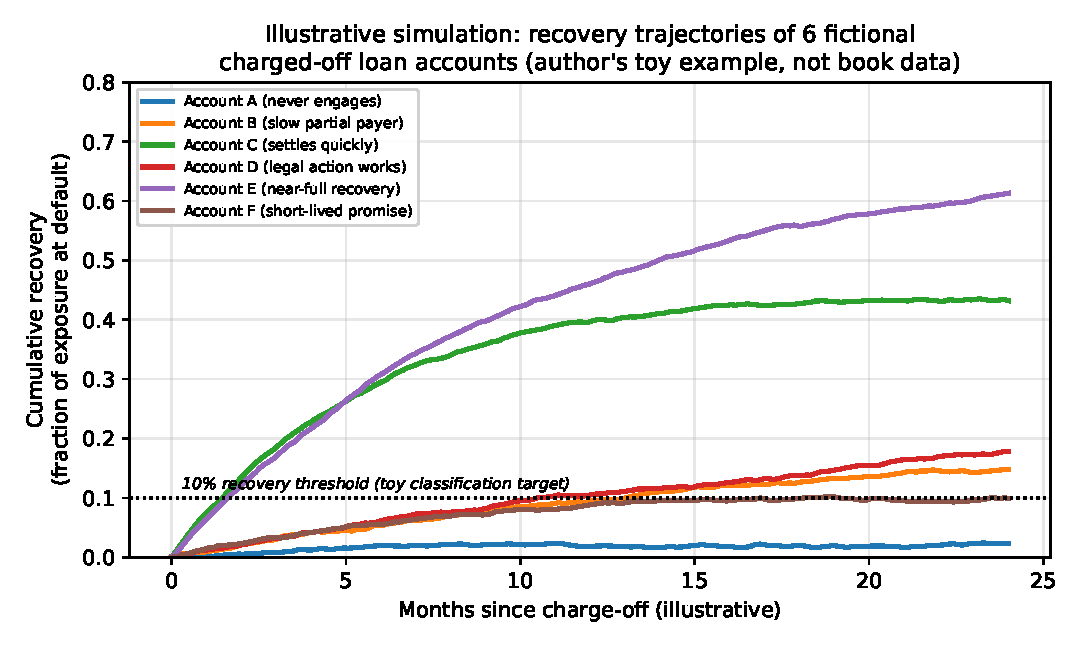
\includegraphics[width=0.85\linewidth]{fig_recovery_curves.pdf}
\end{center}
\end{frame}

\begin{frame}{Toy Running Example: Posterior Summaries}

Fitting the toy BLR model (Sect.~7.2 code) with the from-scratch MALA sampler (Sect.~7.3.1 code) to our 6 fictional accounts gives the following posterior:

\begin{center}
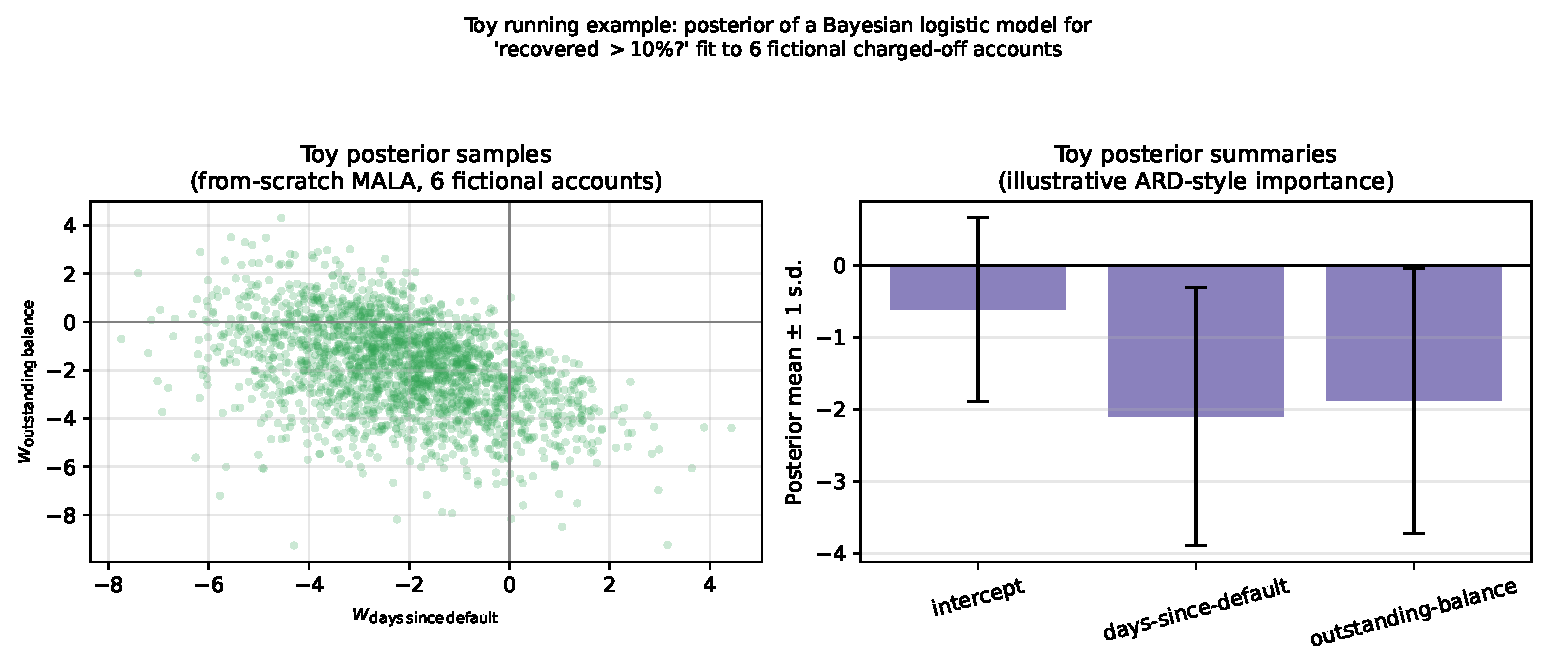
\includegraphics[width=0.95\linewidth]{fig_toy_posterior.pdf}
\end{center}

With only 6 (fictional) data points the posterior is understandably wide -- exactly the kind of honest uncertainty quantification a point-estimate (non-Bayesian) logistic regression would hide from us.
\end{frame}

%%=============================================================================
\section{7.5 Results and Discussions}
%%=============================================================================

\begin{frame}{Sampler Efficiency: Effective Sample Size}

\begin{block}{Raw ESS vs.\ Time-Normalised ESS (book's Lending Club experiments)}
\begin{itemize}
  \item \textbf{Raw ESS}: NUTS $>$ HMC $>$ MALA (roughly 2{,}500 vs.\ 1{,}250 vs.\ under 250 out of 2{,}500 post-burn-in samples). NUTS produces the least autocorrelated samples of the three, exactly as its adaptive trajectory length is designed to achieve.
  \item \textbf{Time-normalised ESS (ESS/time)}: the ranking \emph{flips} -- MALA $>$ HMC $>$ NUTS. MALA has by far the lowest execution time of the three (no Hamiltonian dynamics to simulate), so per unit of wall-clock time it is the most efficient, despite having the worst raw ESS.
  \item Execution-time ranking: MALA fastest, then HMC, then NUTS slowest -- NUTS pays extra wall-clock cost for the on-the-fly trajectory-length tuning (the doubling procedure) on every single iteration.
\end{itemize}
\end{block}

\begin{alertblock}{Key Takeaway}
There is no free lunch: NUTS wins on sample quality per draw, MALA wins on sample quality per second. Which matters more depends on whether wall-clock time or total iteration budget is the binding constraint in practice.
\end{alertblock}
\end{frame}

\begin{frame}{Convergence and Predictive Performance}

\begin{block}{Convergence}
The negative log-likelihood trace plots for all three MCMC methods overlap in the same stable range across thousands of samples -- all three methods have converged to (and are exploring) the same target posterior.
\end{block}

\begin{block}{Predictive Performance (Test-Set AUC)}
\begin{itemize}
  \item MALA: AUC $= 0.6535$ (highest).
  \item NUTS: AUC $= 0.6442$.
  \item HMC: AUC $= 0.6424$ (HMC and NUTS are essentially tied).
\end{itemize}
Interestingly, MALA achieves the \emph{best} predictive performance despite having the \emph{worst} raw ESS -- a reminder that "more effective samples" does not automatically translate into "better point predictions" on a held-out set; posterior predictive averaging can be fairly forgiving of a moderately correlated chain.
\end{block}
\end{frame}

\begin{frame}[allowframebreaks]{Feature Importance: What Drives Recovery?}

\begin{block}{Table 7.1 -- Top-5 Ranked Features per Method (by posterior $\alpha_i$)}
\begin{center}
\small
\begin{tabular}{clll}
\toprule
Rank & MALA & HMC & NUTS \\
\midrule
1 & acc-open-past-24mths & grade & total-bal-il \\
2 & num-actv-rev-tl & purpose & application-type \\
3 & addr-state & home-ownership & annual-inc \\
4 & tot-cur-bal & open-acc & num-rev-accts \\
5 & sub-grade & title & all-util \\
\bottomrule
\end{tabular}
\end{center}
\end{block}

\begin{block}{The Common Thread Across All Three Methods}
Despite ranking different features \#1, all three MCMC methods' top-10 lists repeatedly surface the same handful of themes: \emph{loan purpose}, \emph{title}, \emph{home-ownership status}, \emph{interest rate}, \emph{number of (revolving/bank) accounts}, and \emph{grade}-related variables. The three samplers broadly \emph{agree} on which features matter, even though they disagree on the exact ranking order.
\end{block}

\framebreak

\begin{block}{Does This Make Sense?}
\begin{itemize}
  \item \textbf{Purpose}: a loan taken out for debt consolidation plausibly signals a borrower already under financial strain -- higher default risk, and (conditional on default) lower odds of meaningful recovery -- versus, say, a home-improvement loan.
  \item \textbf{Interest rate}: higher rates are charged to riskier borrowers, who are correspondingly less likely to have the means to repay after default.
  \item \textbf{Home ownership / grade}: proxies for overall financial stability and creditworthiness that plausibly correlate with post-default collectability.
\end{itemize}
This qualitative face-validity is itself a useful sanity check on an otherwise ``black-box-feeling'' ARD ranking.
\end{block}

\end{frame}

%%=============================================================================
\section{7.6 Conclusion}
%%=============================================================================

\begin{frame}[allowframebreaks]{7.6 Conclusion}

\begin{block}{What This Chapter Did}
\begin{itemize}
  \item First-in-literature application of a Bayesian inference framework (BLR-ARD) to detect \emph{presence} of recovery on charged-off peer-to-peer lending accounts.
  \item Trained the same model with three MCMC samplers -- MALA, HMC, and NUTS -- under a matched experimental protocol.
\end{itemize}
\end{block}

\begin{block}{What Was Found}
\begin{itemize}
  \item \textbf{Speed}: MALA fastest, HMC in the middle, NUTS slowest (extra cost of on-the-fly trajectory tuning).
  \item \textbf{Raw ESS}: NUTS highest, HMC second, MALA lowest.
  \item \textbf{Time-normalised ESS}: MALA wins, NUTS is the laggard -- the exact opposite ranking to raw ESS.
  \item \textbf{Predictive performance (AUC)}: MALA best, HMC and NUTS statistically similar to one another.
  \item \textbf{Feature relevance}: all three MCMC methods broadly agree that \emph{purpose}, \emph{home-ownership}, and \emph{interest rate} are among the most important drivers of whether a charged-off account will show recovery.
\end{itemize}
\end{block}

\framebreak

\begin{block}{Limitations and Future Work (as noted by the authors)}
\begin{itemize}
  \item This chapter only detects \emph{whether} recovery happens (binary), not \emph{how much} is recovered -- modelling the actual continuous recovery amount with Bayesian techniques remains unexplored in the literature and is flagged as future work.
  \item More complex models (e.g.\ deep neural networks) could be substituted for BLR-ARD within the same Bayesian/MCMC training framework.
\end{itemize}
\end{block}

\begin{alertblock}{Looking Ahead}
The next chapter turns to Bayesian evidence metrics based on normalizing flows, applied to selecting and comparing models that predict audit outcomes for South African municipalities.
\end{alertblock}

\end{frame}

\end{document}
